\documentclass[12pt, a4paper]{article}
\usepackage[T2A]{fontenc}
\usepackage[utf8]{inputenc}
\usepackage[english,ukrainian]{babel}
\usepackage{amsmath, amssymb}
\usepackage{verbatim}
\usepackage{minted}
\usepackage{euler}

\usepackage[top = 1.5 cm, left = .75 cm, right = .75 cm, bottom = 1.5 cm]{geometry}
\usepackage[unicode = true, colorlinks = true, linktoc = all, linkcolor = blue]{hyperref}
\usepackage{subcaption}

\usepackage{float}
\usepackage{graphicx}

\usepackage{amsthm}
\newtheorem{lemma}{Лема}
\newtheorem*{lemma*}{Лема}
\newtheorem{theorem}{Теорема}
\newtheorem*{theorem*}{Теорема}
\newtheorem{definition}{Визначення}
\newtheorem*{definition*}{Визначення}
\theoremstyle{definition}
\newtheorem{remark}{Зауваження}
\newtheorem*{remark*}{Зауваження}
\newtheorem{example}{Приклад}
\newtheorem*{example*}{Приклад}
\newtheorem{problem}{Задача}
\newtheorem*{problem*}{Задача}
\newtheorem{solution}{Розв'язок}
\newtheorem*{solution*}{Розв'язок}
\newtheorem{corollary}{Наслідок}
\newtheorem*{corollary*}{Наслідок}

\newcommand{\NN}{\mathbb{N}}
\newcommand{\RR}{\mathbb{R}}
\newcommand{\CC}{\mathbb{C}}
\newcommand{\HH}{\mathcal{H}}
\newcommand{\Max}{\displaystyle\max\limits}
\newcommand{\Sup}{\displaystyle\sup\limits}
\newcommand{\Sum}{\displaystyle\sum\limits}
\newcommand{\Prod}{\displaystyle\prod\limits}
\newcommand{\Int}{\displaystyle\int\limits}
\newcommand{\Iint}{\displaystyle\iint\limits}
\newcommand{\Lim}{\displaystyle\lim\limits}

\newcommand*\diff{\mathop{}\!\mathrm{d}}

\newcommand{\degrees}{^\circ}

\renewcommand{\bf}[1]{\textbf{#1}}
\renewcommand{\epsilon}{\varepsilon}
\renewcommand{\phi}{\varphi}

\newcommand{\ol}[1]{\overline{#1}}
\newcommand{\ul}[1]{\underline{#1}}

\DeclareMathOperator{\signum}{sign}
\DeclareMathOperator{\diam}{diam}
\DeclareMathOperator{\rang}{rang}
\DeclareMathOperator{\const}{const}
\DeclareMathOperator{\cond}{cond}
\DeclareMathOperator{\diagonal}{diag}

\DeclareMathOperator*{\Min}{min}

\setlength\parindent{0pt}
\allowdisplaybreaks

\newcommand{\cover}[2]{
\begin{center}
\hfill \break
  М{\footnotesizeІНІСТЕРСТВО ОСВІТИ ТА НАУКИ} У{\footnotesizeКРАЇНИ} \\
  К{\footnotesizeИЇВСЬКИЙ НАЦІОНАЛЬНИЙ УНІВЕРСИТЕТ ІМЕНІ} Т{\footnotesizeАРАСА} Ш{\footnotesizeЕВЧЕНКА} \\ 
  Ф{\footnotesizeАКУЛЬТЕТ КОМП'ЮТЕРНИХ НАУК ТА КІБЕРНЕТИКИ} \\
  К{\footnotesizeАФЕДРА ОБЧИСЛЮВАЛЬНОЇ МАТЕМАТИКИ}
\end{center}

\vfill 

\begin{center}
  \large{
    Звіт до лабораторної роботи №{#1} на тему: \\ 
    \guillemotleft{}{#2}\guillemotright{}
  }
\end{center}

\vfill 

\begin{flushright}
  Виконав студент групи ОМ-4 \\
  Скибицький Нікіта
\end{flushright}

\vfill 

\begin{center}
    Київ, 2019
\end{center}

\thispagestyle{empty} 
\newpage
}

\newenvironment{system}{%
  \begin{equation}%
    \left\{%
      \begin{aligned}%
}{%
      \end{aligned}%
    \right.%
  \end{equation}%
}
\newenvironment{system*}{%
  \begin{equation*}%
    \left\{%
      \begin{aligned}%
}{%
      \end{aligned}%
    \right.%
  \end{equation*}%
}

\newcommand{\pluseqq}{{\:\:+\!\!=\:\:}}
.sty}

\begin{document}

\cover{1}{Чисельне розв'язування крайових задач математичної фізики. \\ Проекційні та варіаційні методи}

\tableofcontents

\numberwithin{equation}{section}
\section{Постановка задачі}

\subsection{Загальна постановка задачі}

Знайти наближений розв'язок наступної задачі проекційним та варіаційним методами: задано рівняння
\begin{equation}
    \label{eq:1.1}
    - \frac{\diff}{\diff x} \left( k(x) \cdot \frac{\diff u(x)}{\diff x} \right) + p(x) \cdot \frac{\diff u(x)}{\diff x} + q(x) \cdot u(x) = f(x), \quad a < x < b,
\end{equation}
з крайовими умовами
\begin{align}
    \label{eq:1.2}
    -k(x) \cdot \frac{\diff u(x)}{\diff x} + \alpha_1 u(x) &= \mu_1, \quad x = a, \\
    \label{eq:1.3}
    k(x) \cdot \frac{\diff u(x)}{\diff x} + \alpha_2 u(x) &= \mu_2, \quad x = b,
\end{align}
де
\begin{align}
    \label{eq:1.4}
    k(x) &= k_1 \sin(k_2 x) + k_3, \\
    & \quad k(x) > 0, \nonumber \\
    \label{eq:1.5}
    p(x) &= p_1 \cos(p_2 x) + p_3, \\
    \label{eq:1.6}
    q(x) &= q_1 \sin(q_2 x) + q_3, \\
    & \quad q(x) \ge 0, \nonumber \\
    & \quad \alpha_1, \alpha_2 > 0. \nonumber
\end{align}

\subsubsection{Зауваження}

Задача \emph{модельна}, тому функцію $f(x)$ і константи $\mu_1$, $\mu_2$ виражаємо з відповідних рівностей:
\begin{align}
    \label{eq:1.7}
    f(x) &= -(k(x) \cdot u'(x))' + p(x) \cdot u'(x) + q(x) \cdot u(x), \\
    \label{eq:1.8}
    \mu_1 &= -k(a) \cdot u'(a) + \alpha_1 u(a), \\
    \label{eq:1.9}
    \mu_2 &= k(b) \cdot u'(b) + \alpha_2 u(b),
\end{align}
де $u(x)$ --- точний розв'язок задачі, функція $u(x) = m_1 \sin(m_2 x) + m_3$.

\subsection{Параметри варіанту}

\begin{table}[H]
    \centering
    \begin{tabular}{|c|c||c|c||c|c|c||c|c|c||c|c|c||c|c|c|}
        \hline
        $a$ & $b$ & $\alpha_1$ & $\alpha_2$ & $k_1$ & $k_2$ & $k_3$ & $p_1$ & $p_2$ & $p_3$ & $q_1$ & $q_2$ & $q_3$ & $m_1$ & $m_2$ & $m_3$ \\ \hline
        0 & 4 & 4 & 2 & 2 & 3 & 1 & 2 & 1 & 1 & 0 & 2 & 3 & 2 & 2 & 1 \\ \hline
    \end{tabular}
\end{table}

\subsection{Методи}

Використати проекційний \emph{метод колокацій} та варіаційний \emph{метод Рітца}. 

\section{Теоретичні відомості}

\setcounter{subsection}{-1}
\subsection{Аналітичні маніпуляції}

Перш за все, виразимо функцію $f(x)$ і константи $\mu_1$, $\mu_2$ з рівностей \eqref{eq:1.7}--\eqref{eq:1.9}:
\begin{align}
    \label{eq:2.0.1}
    f(x) &= 3 + 14 \sin(2 x) + 4 \cos(2 x) + 4 \cos(3 x) - 20 \cos(5 x), \\
    \label{eq:2.0.2}
    \mu_1 &= 0, \\
    \label{eq:2.0.3}
    \mu_2 &= 6.
\end{align}

\subsubsection{Однорідні крайові умови}

Зведемо крайові умови до однорідних. Для цього знайдемо представлення
\begin{equation}
    \label{eq:2.0.4}
    u(x) = \phi_0(x) + v(x),
\end{equation}
де функція $\phi_0(x)$ задовольняє неоднорыдним крайовим умовам, а функція $v(x)$ --- однорідним крайовим умовам
\begin{align}
    \label{eq:2.0.5}
    0 &= -k(a) \cdot u'(a) + \alpha_1 u(a), \\
    \label{eq:2.0.6}
    0 &= k(b) \cdot u'(b) + \alpha_2 u(b).
\end{align}

Шукатимемо $\phi_0(x)$ у вигляді
\begin{equation}
    \label{eq:2.0.7}
    \phi_0(x) = C x + D.
\end{equation}

Константи $C$, $D$ знайдемо із співвідношень \eqref{eq:1.2},  \eqref{eq:1.3}. Отримаємо наступну систему:
\begin{align}
    \label{eq:2.0.8}
    C (\alpha_1 a - k(a)) + \alpha_1 D &= \mu_1, \\
    \label{eq:2.0.9}
    C (\alpha_2 b - k(b)) + \alpha_2 D &= \mu_2.
\end{align}

Її розв'язок
\begin{equation}
    \label{eq:2.0.10}
    C = \texttt{0.7120099335017387}, \quad D = \texttt{0.17800248337543467}.
\end{equation}

\subsubsection{Координатна система функцій}

В якості системи координатних функцій оберемо:
\begin{align}
    \label{eq:2.0.11}
    \phi_1(x) &= (x - a)^2 (x - c), \\
    \label{eq:2.0.12}
    \phi_2(x) &= (x - d) (b - x)^2, \\
    \label{eq:2.0.13}
    \phi_n(x) &= (x - a)^2 (b - x)^{n - 1}, \quad n \ge 3,
\end{align}
де $c$, $d$ --- такі константи, що $\phi_1$, $\phi_2$ задовольняють однорідним крайовим умовам \eqref{eq:2.0.5}, \eqref{eq:2.0.6}, а саме
\begin{align}
     \label{eq:2.0.14}
     c &= b + \frac{k(b) (b - a)}{2 k(b) + \alpha_2 (b - a)}, \\
     \label{eq:2.0.15}
     d &= a - \frac{k(a) (b - a)}{2 k(a) + \alpha_1 (b - a)}.
\end{align}

В результаті обчислень отримуємо:
\begin{equation}
    \label{eq:2.0.16}
    c = \texttt{3.96274583524315}, \quad d = \texttt{-0.222222222222222}.
\end{equation}


\numberwithin{equation}{subsection}
\subsection{Метод колокацій}

Розглянемо загальне рівняння
\begin{equation}
    \label{eq:2.1.1}
    A u = f,
\end{equation}
де $A: E \to F$. Замінимо його на рівняння
\begin{equation}
    \label{eq:2.1.2}
    P_n(A u_n) = P_n f,
\end{equation}
або на
\begin{equation}
    \label{eq:2.1.3}
    P_n (A u_n - f) = 0.
\end{equation}

Координатну систему візьмемо $\{\phi_i\} \in D(A) \subseteq E$, а проекційну --- $\{\psi_i\} \in F^\star$. % тобто $\psi_i$ --- лінійні функціонали.
Тоді можемо останню рівність переписати у вигляді
\begin{equation}
    \label{eq:2.1.4}
    \psi_j (A u_n - f) = 0,
\end{equation}
або ж, що те саме,
\begin{equation}
    \label{eq:2.1.5}
    \psi_j (A u_n) = \psi_j f.
\end{equation}

Шукачи розв'язок у вигляді
\begin{equation}
    \label{eq:2.1.6}
    u_n = \sum_{i = 1}^n c_i \phi_i,
\end{equation}
матимемо
\begin{equation}
    \label{eq:2.1.7}
    \psi_j \left( A \left( \sum_{i = 1}^n c_i \phi_i \right) \right) = \psi_j f, \quad j = \overline{1, n},
\end{equation}
або ж, враховучи лінійність $A$ і $\psi_j$,
\begin{equation}
    \label{eq:2.1.8}
    \sum_{i = 1}^n c_i \psi_j (A \phi_i) = \psi_j f, \quad j = \overline{1, n}.
\end{equation}

У матричному вигляді, систему вище можна записати як
\begin{equation}
    \label{eq:2.1.9}
    \begin{pmatrix}
        \psi_1 (A \phi_1) & \psi_1 (A \phi_2) & \cdots & \psi_1 (A \phi_n) \\
        \psi_2 (A \phi_1) & \psi_2 (A \phi_2) & \cdots & \psi_2 (A \phi_n) \\
        \vdots & \vdots & \ddots & \vdots \\
        \psi_n (A \phi_1) & \psi_n (A \phi_2) & \cdots & \psi_n (A \phi_n)
    \end{pmatrix}
    \begin{pmatrix}
        c_1 \\ c_2 \\ \vdots \\ c_n
    \end{pmatrix}
    =
    \begin{pmatrix}
        \psi_1 f \\ \psi_2 f \\ \vdots \\ \psi_n f
    \end{pmatrix}
\end{equation}

Якщо взяти у якості $\{\psi_j\}$ систему функцій Чебишова, то отримаємо, що визначник цієї системи не рівний нулеві.

\subsection{Метод Рітца}

Нехай, як і раніше, ми розв'язуємо рівняння
\begin{equation}
    \label{eq:2.2.1}
    A u = f,
\end{equation}
де $A: H \to H$, $H$ --- дійсний гільбертовий простір. Нагадаємо, що ми ставимо цій задачі й відповідність задачу мінімізації
\begin{equation}
    \label{eq:2.2.2}
    \inf_{u \in D(A)} \Phi(u) = \Phi(u^\star) = u_0.
\end{equation}

Нехай також виконуються певні припущення, необхідні для збіжності, а саме:
\begin{enumerate}
    \item $A$ --- симетричний (самоспряжений), тобто
    \begin{equation}
        \label{eq:2.2.3}
        (A u, v) = (u, A v).
    \end{equation}
    
    \item $A$ --- додатно визначений, тобто
    \begin{equation}
        \label{eq:2.2.4}
        \exists \mu > 0: \forall u \in D(A) \quad (A u, u) \ge \mu \|u\|^2 (u, A v).
    \end{equation}
    
    \item $f \in R(A)$ --- область значень оператора $A$.
\end{enumerate}

\subsubsection{Мінімізаційна послідовність}

\begin{enumerate}
    \item Як і раніше, нехай $\{\phi_i\} \in D(A)$ --- повна;
    \item Ввводимо простір $H_n = \mathcal{L}(\phi_1, \ldots, \phi_n)$;
    \item Розв'язок шукаємо у вигляді $u_n = \sum_{i = 1}^n c_i \phi_i$.
\end{enumerate}

Наш загальний функціонал Рітца
\begin{equation}
    \label{eq:2.2.5}
    \inf_{u \in H_n} \Phi(u) = \Phi(u_n)
\end{equation}
з функцією $G$ вигляду
\begin{equation}
    \label{eq:2.2.6}
    G(u_n, v) = (f, v), \quad \forall v \in H_n,
\end{equation}
або, що те саме у наших умовах,
\begin{equation}
    \label{eq:2.2.7}
    G(u_n, \phi_j) = (f, \phi_j), \quad j = \overline{1, n},
\end{equation}
можна буде записати у вигляді
\begin{equation}
    \label{eq:2.2.8}
    \sum_{i = 1}^n c_i G(\phi_i, \phi_j) = (f, \phi_j), \quad j = \overline{1, n},
\end{equation}
або, що те саме в наших умовах,
\begin{equation}
    \label{eq:2.2.9}
    \sum_{i = 1}^n c_i (A \phi_i, \phi_j) = (f, \phi_j), \quad j = \overline{1, n}.
\end{equation}

Мінімізаційна послідовність звелася до тієї ж системи що й у методі Бубнова-Гальоркіна, то які ж його переваги?

\subsection{Метод Рітца в \texorpdfstring{$H_A$}{HA}}

Справа в тому, що якщо оператор $A$ задовольняє умовам \eqref{eq:2.2.3} і \eqref{eq:2.2.4}, то можна ввести енергетичний простір $H_A$ у якому скалярний добуток і норму введено за формулами
\begin{equation}
    \label{eq:2.3.1}
    (u, v)_A = (A u, u), \quad \|u\|_A^2 = (u, u)_A.
\end{equation}

Можна перевірити, що ці функції задовольняють аксіомам скалярного добутку та норми. Таким чином $H_A$ --- гільбертовий простір, ширший за $D(A)$. \medskip

Тоді задачі \eqref{eq:2.2.1} ставимо у відповідність задачу
\begin{equation}
    \label{eq:2.3.2}
    \inf_{u \in H_A} \Phi(u) = \Phi(u_n),
\end{equation}
для якої мають місце аналогічні результати:

\begin{theorem}
    Виконуються наступні співвідношення:
    \begin{enumerate}
        \item \begin{equation}
            \label{eq:2.3.3}
            \Phi(u) = (A u, u) - 2 (f, u) = \|u - u^\star\|_A^2 - \|u^\star\|_A^2,
        \end{equation}
        
        \item \begin{equation}
            \label{eq:2.3.4}
            \inf_{u \in H_n \subset H_A} \Phi(u) = \Phi(u_n) = \Phi_0.
        \end{equation}
    \end{enumerate}
\end{theorem}

З останнього співвідношення маємо
\begin{equation}
    \label{eq:2.3.5}
    (A u_n, v) = (f, v), \quad v \in H_n,
\end{equation}
тоді
\begin{equation}
    \label{eq:2.3.6}
    (A u_n - A u^\star, v) = 0, \quad v \in H_n,
\end{equation}
або ж, що те саме,
\begin{equation}
    \label{eq:2.3.7}
    (u_n - u^\star, v)_A = 0, \quad v \in H_n.
\end{equation}

Це означає, що
\begin{equation}
    \label{eq:2.3.8}
    u = P_{H_n} u^\star.
\end{equation}

\begin{theorem}
    Нехай координатна система $\{\phi_i\}$ є повною в $H_A$, тоді при $n \to \infty$ мінімізуюча послідовність $\{u_n\}$ метода Рітца збігається до розв'язку задачі \eqref{eq:2.2.1} в нормі простору $H_A$.
\end{theorem}

\begin{minipage}[t]{.475\textwidth}
    \begin{example*}
    $\{\phi_i\}_{i = 1}^{n - 1}$ --- так звані штафетини:
        \begin{equation}
        \label{eq:2.3.9}
            \phi_i(x) = \begin{cases}
                \frac{x - x_{i - 1}}{h_i}, & x_{i - 1} \le x \le x_i, \\[.5ex]
                \frac{x_{i + 1} - x}{h_i}, & x_i \le x \le x_{i + 1}, \\
                0, & x \not\in [x_{i - 1}, x_{i + 1}].
            \end{cases}
        \end{equation}
        А також $\phi_0, \phi_n$ --- напівштафетини, у яких обрізані половини, які виходять за $[x_0, x_n]$,
        \begin{align*}
            \phi_0(x) &= \begin{cases}
                \frac{x_1 - x}{h_i}, & x_0 \le x \le x_1, \\
                0, & x_1 \le x.
            \end{cases} \\
            \phi_n(x) &= \begin{cases}
                0, & x_{n - 1} \le x, \\
                \frac{x - x_{n - 1}}{h_i}, & x_{n - 1} \le x \le x_n.
            \end{cases}
        \end{align*}
    \end{example*}
\end{minipage}
\begin{minipage}[t]{.05\textwidth}
    $\left.\right.$
\end{minipage}
\begin{minipage}[t]{.475\textwidth}
    Графіки цих функцій мають вигляд
    \begin{figure}[H]
        \centering
        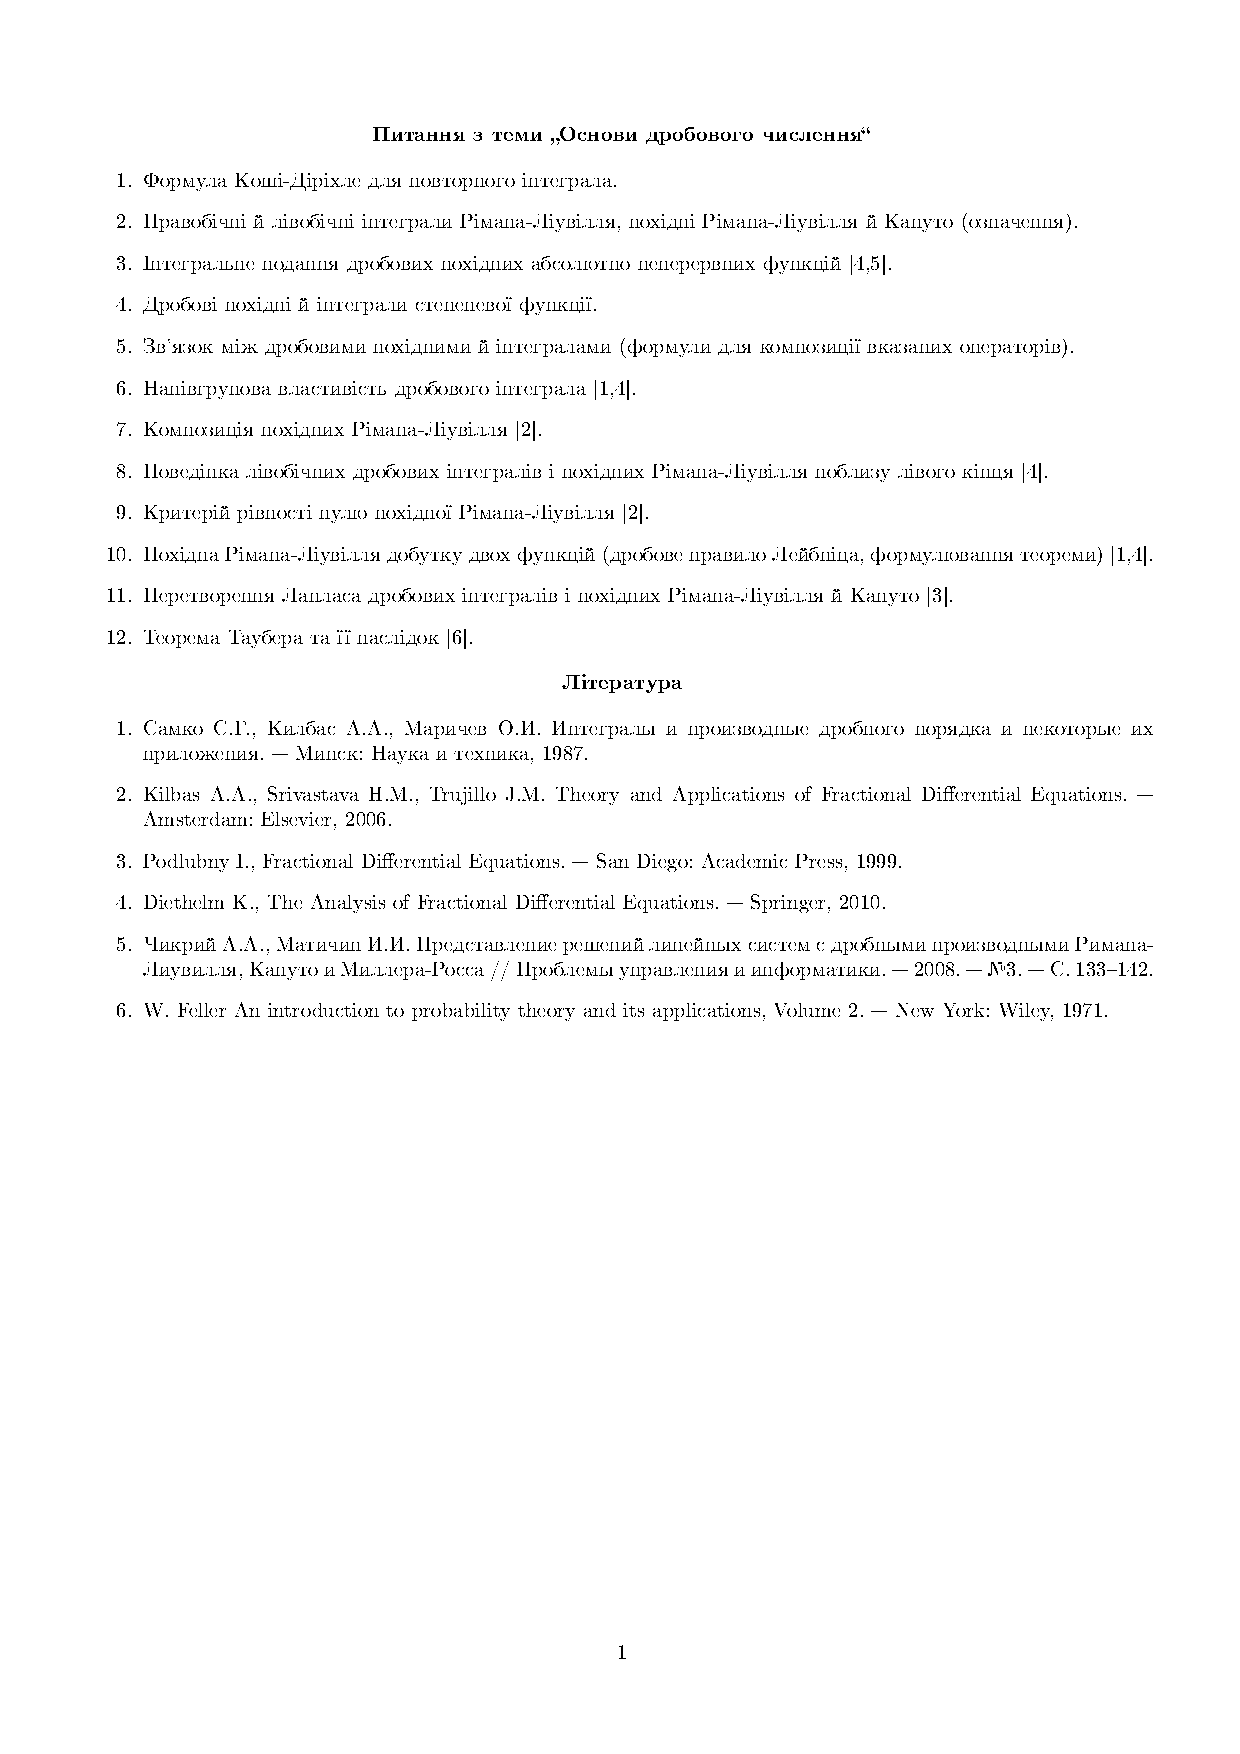
\includegraphics[width=.789473684\textwidth]{1.mps} % .375 of entire textwidth
        \caption{``штафетина'' від $x_{i - 1}$ до $x_{i + 1}$.}
    \end{figure}
\end{minipage}

\section{Чисельне моделювання}

Було використано мову програмування \verb|python| і бібліотеки \verb|sympy| (для символьних обчислень), \verb|numpy| (для ефективного розв'язування систем лінійних алгебраїчних рівнянь, що виникають, а також \verb|matplotlib| (для побудови графіків).

\subsection{Похибки}
Відхилення від точного розв'язку в нормі 
\begin{equation}
    \|f\| = \frac{1}{b - a} \int_a^b f^2(x) \diff x:
\end{equation}
\begin{itemize}
    \item Колокацій, 8 функцій: \texttt{0.0025116018874234433};
    \item Колокацій, 16 функцій: \texttt{1.1242967189129815e-05};
    \item Рітца, 4 функції: \texttt{0.5227343590104221};
    \item Рітца, 8 функцій: \texttt{1.0763937437329292e-06}.
\end{itemize}

Бачимо, що метод Рітца збігається швидше.

\subsection{Графіки}
\begin{figure}[H]
    \begin{subfigure}{.5\textwidth}
    \centering
    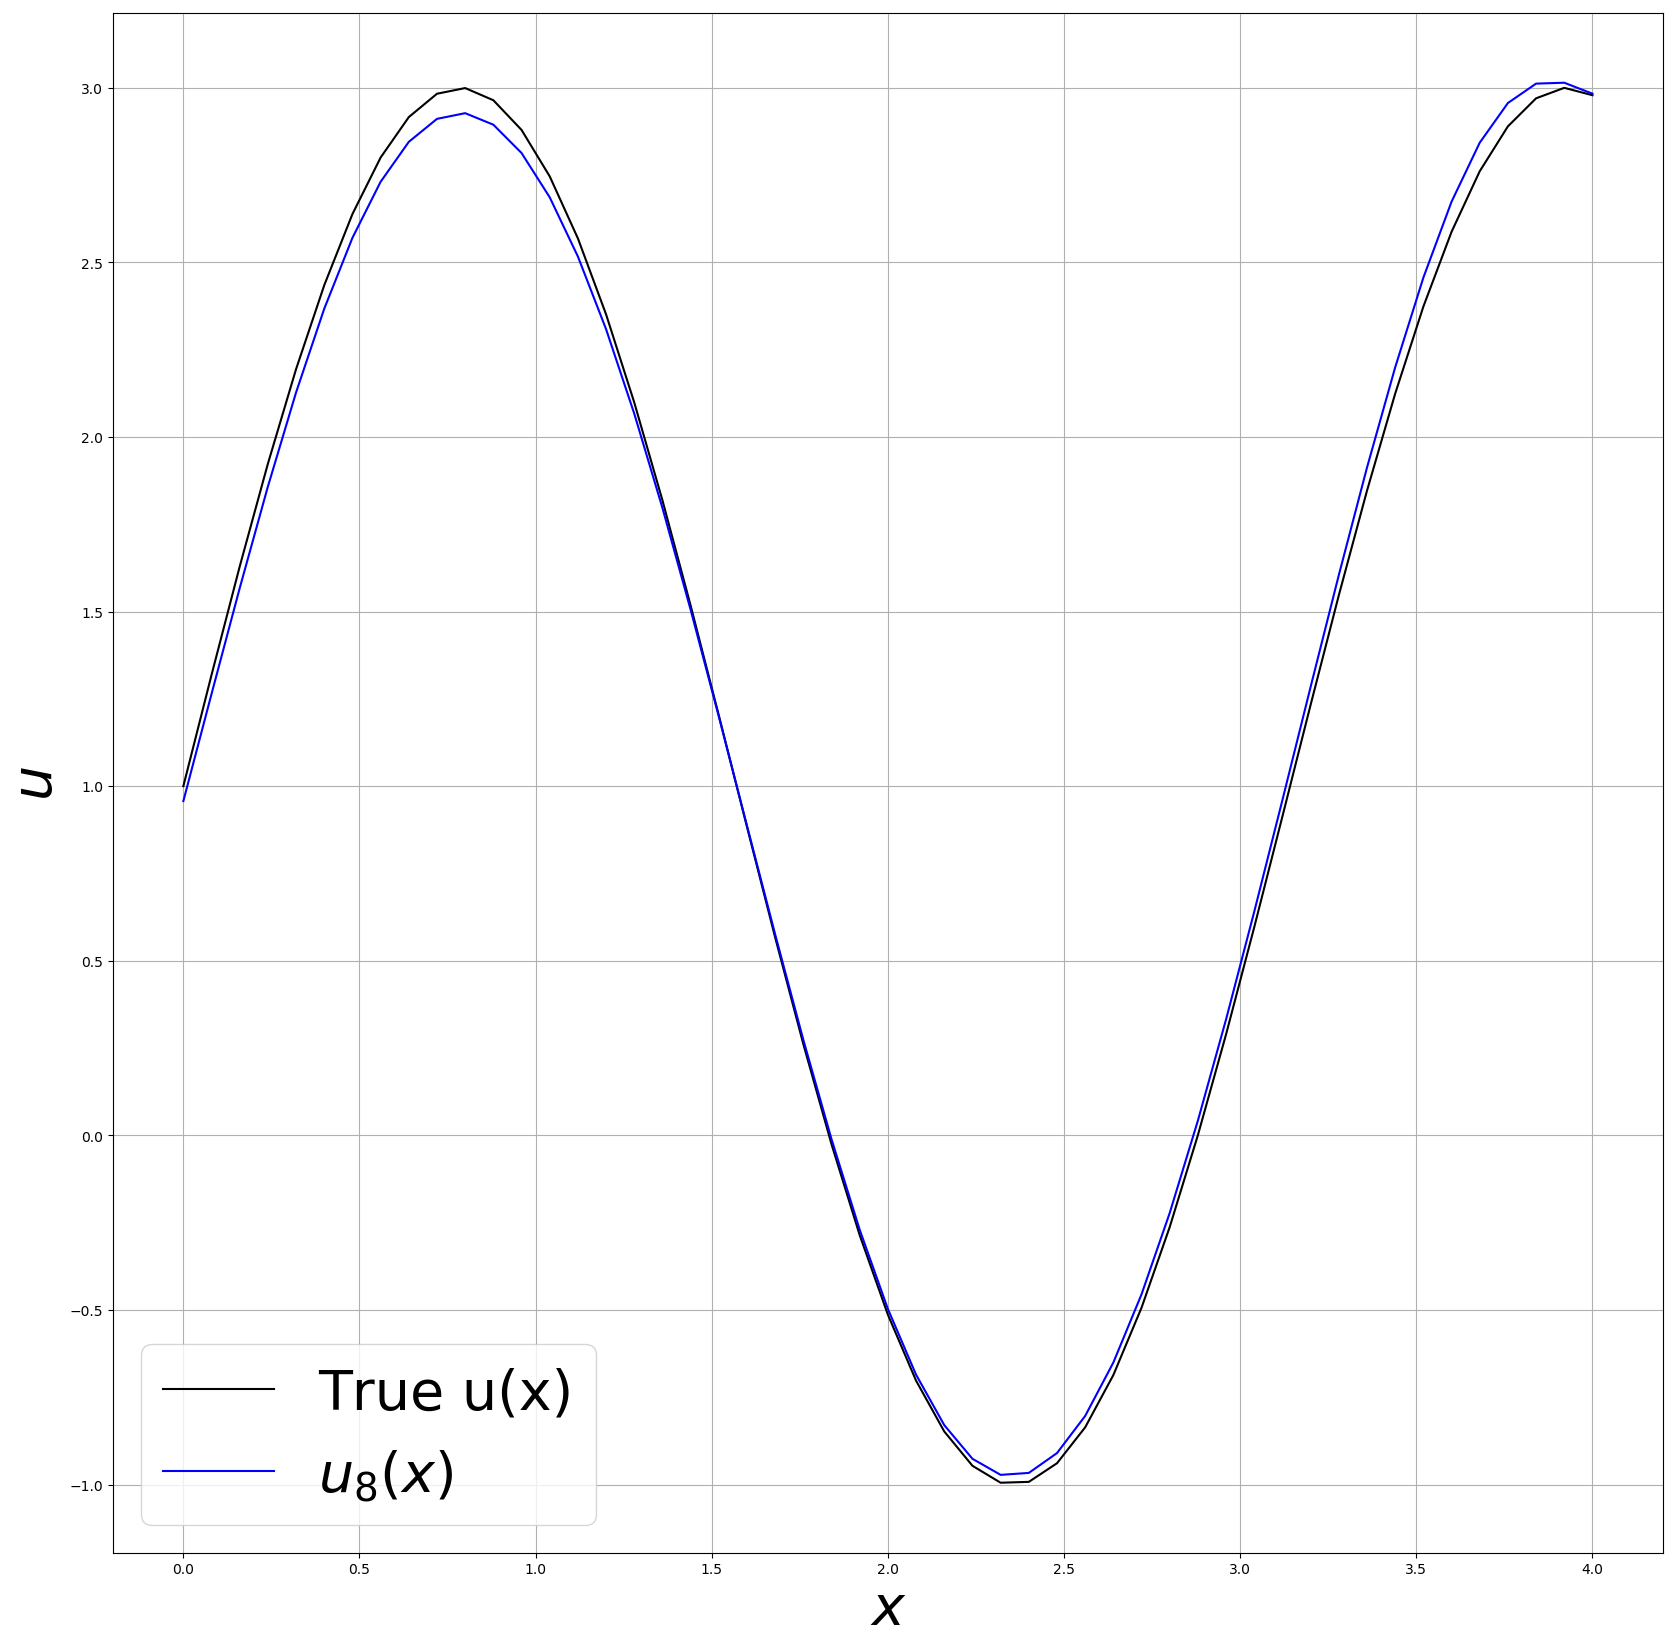
\includegraphics[width=.95\linewidth]{collocation_8.png}
    \caption{Колокацій, 8 функцій}
    \end{subfigure}
    \hfill
    \begin{subfigure}{.5\textwidth}
    \centering
    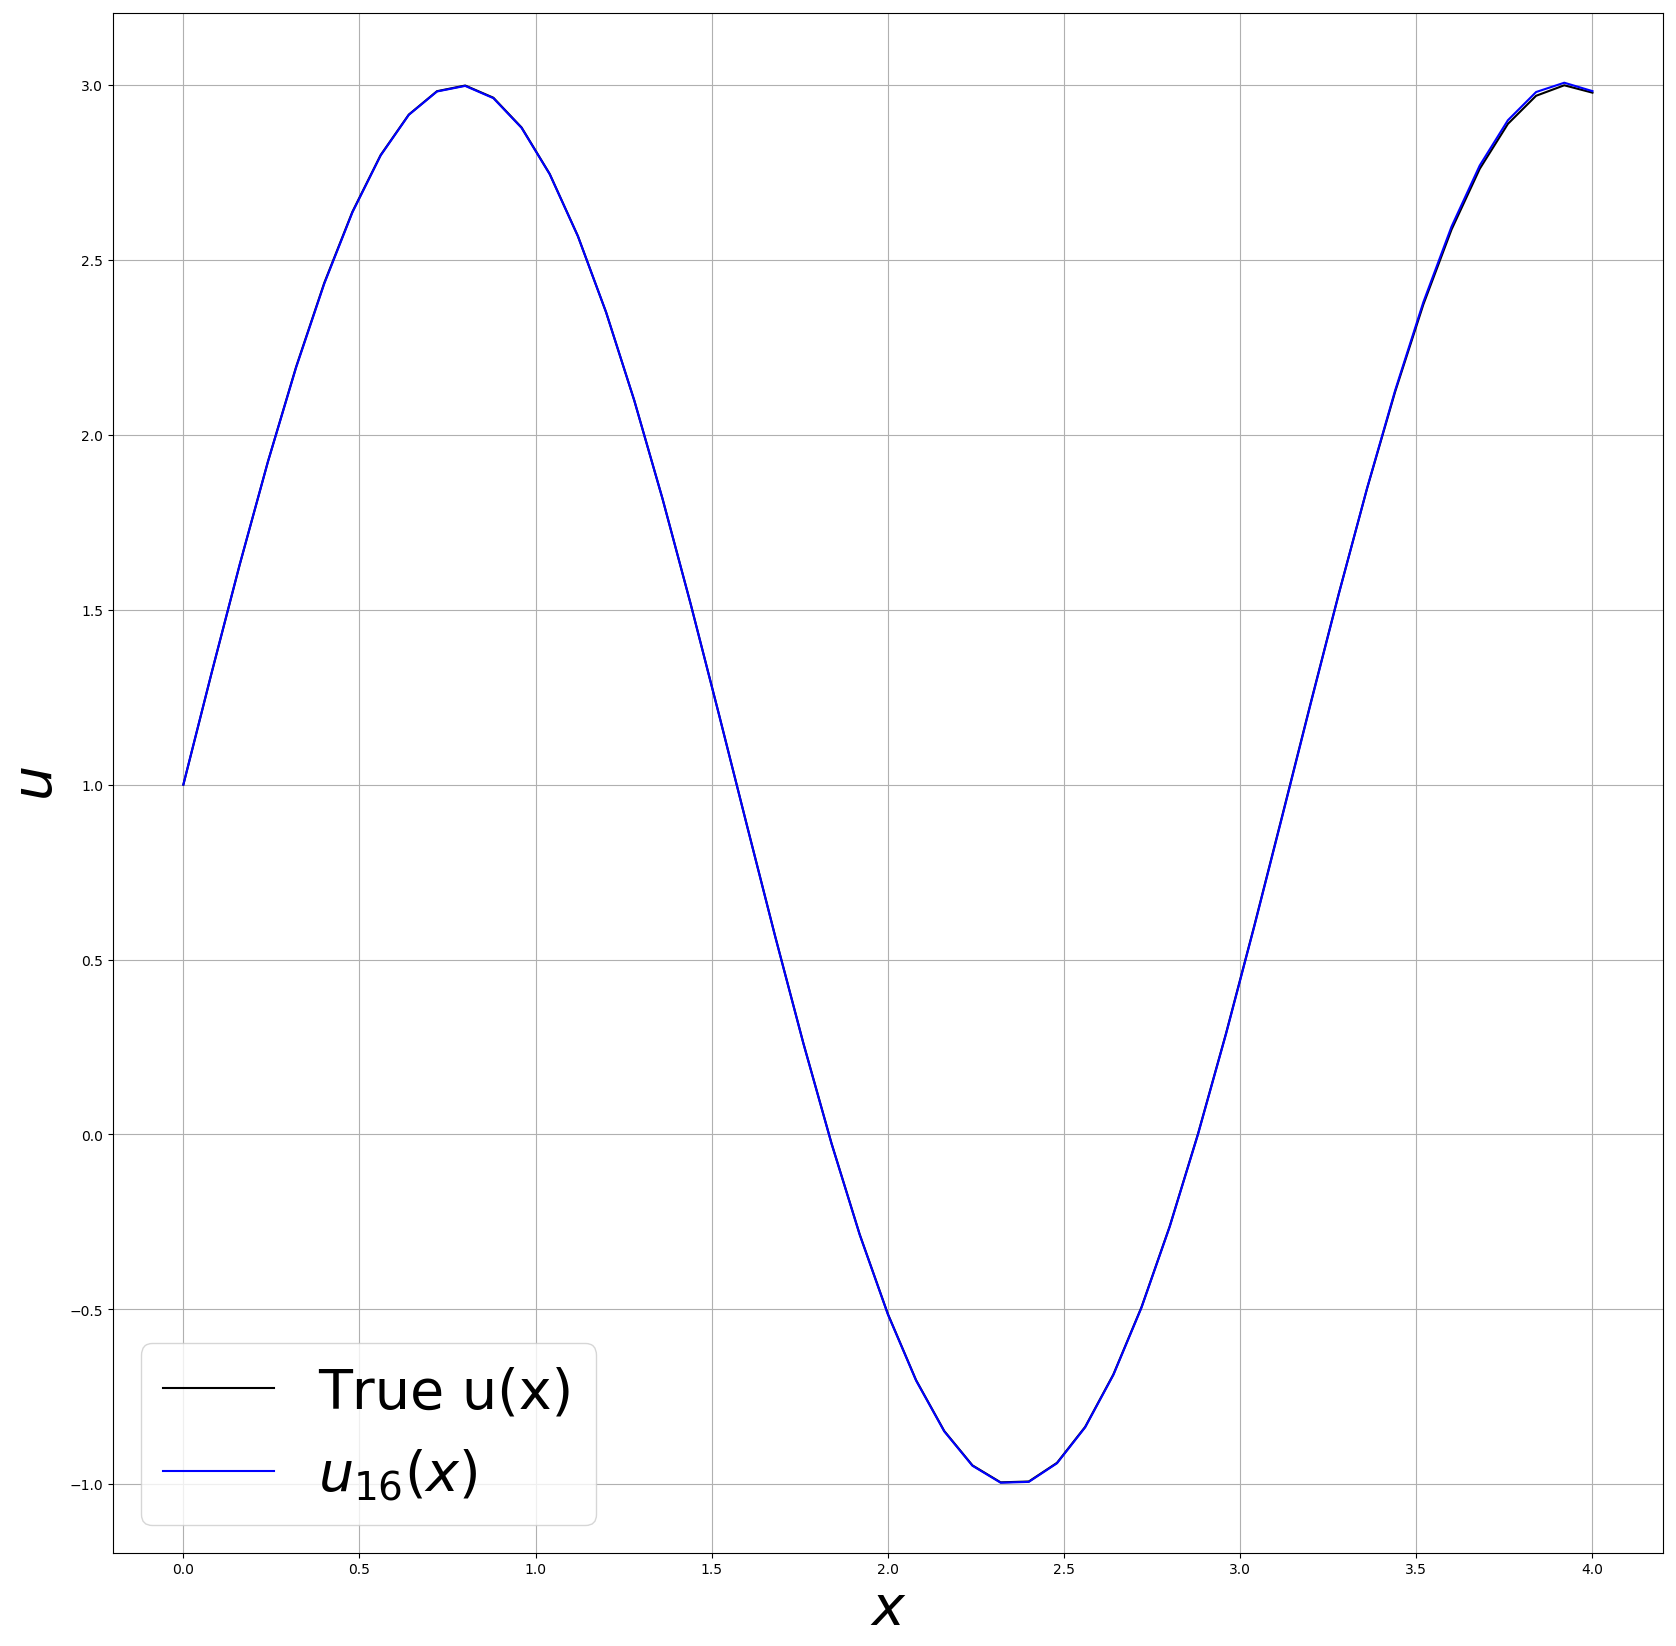
\includegraphics[width=.95\linewidth]{collocation_16.png}
    \caption{Колокацій, 16 функцій}
    \end{subfigure}
    \hfill
    \begin{subfigure}{.5\textwidth}
    \centering
    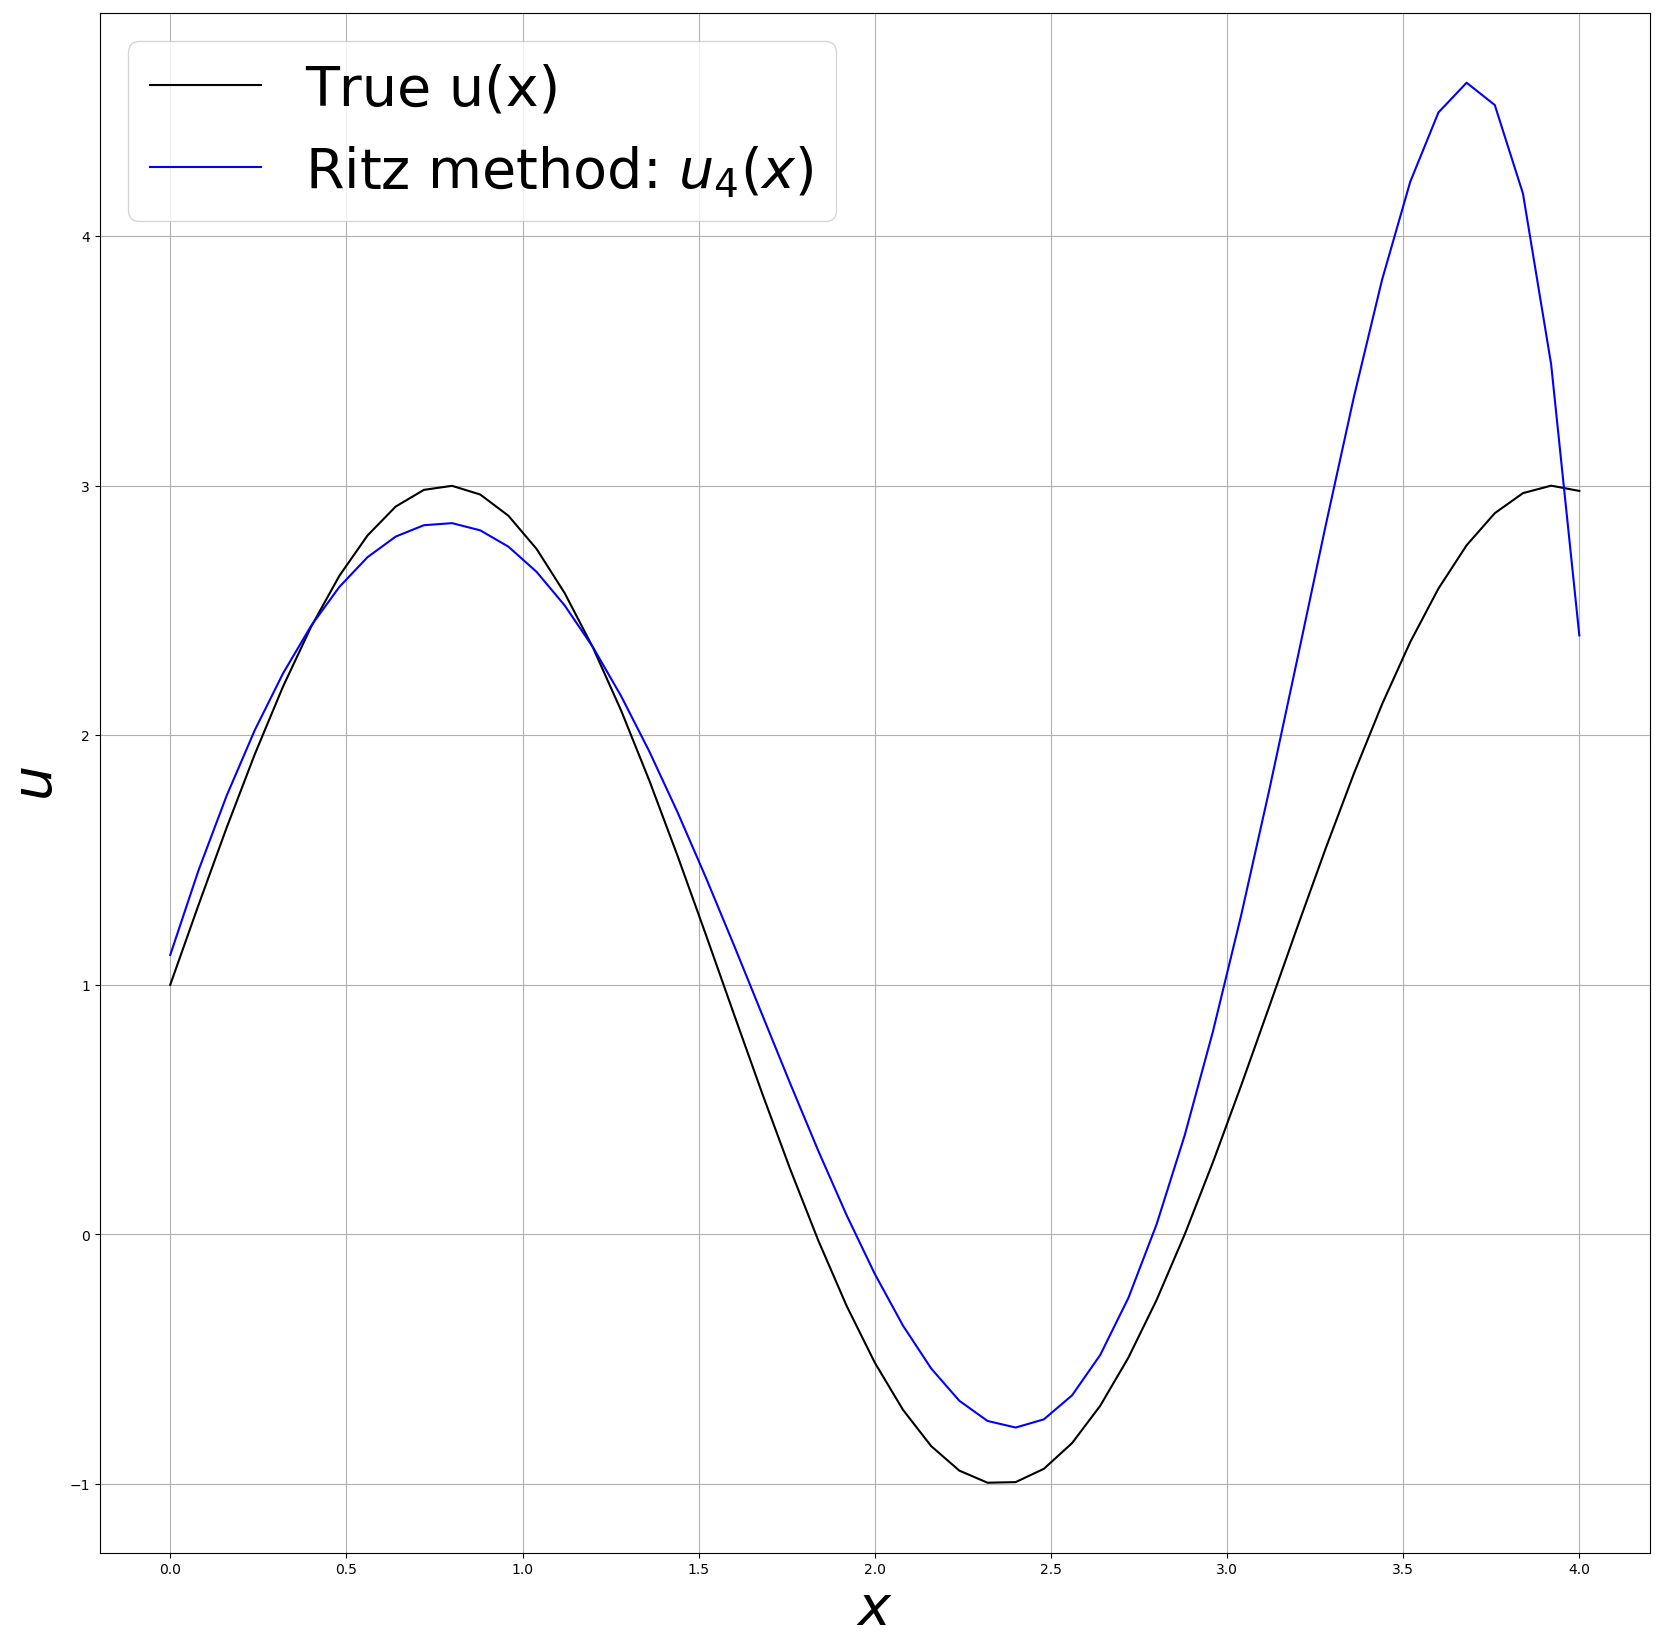
\includegraphics[width=.95\linewidth]{ritz_4.png}
    \caption{Рітца, 4 функції}
    \end{subfigure}
    \begin{subfigure}{.5\textwidth}
    \centering
    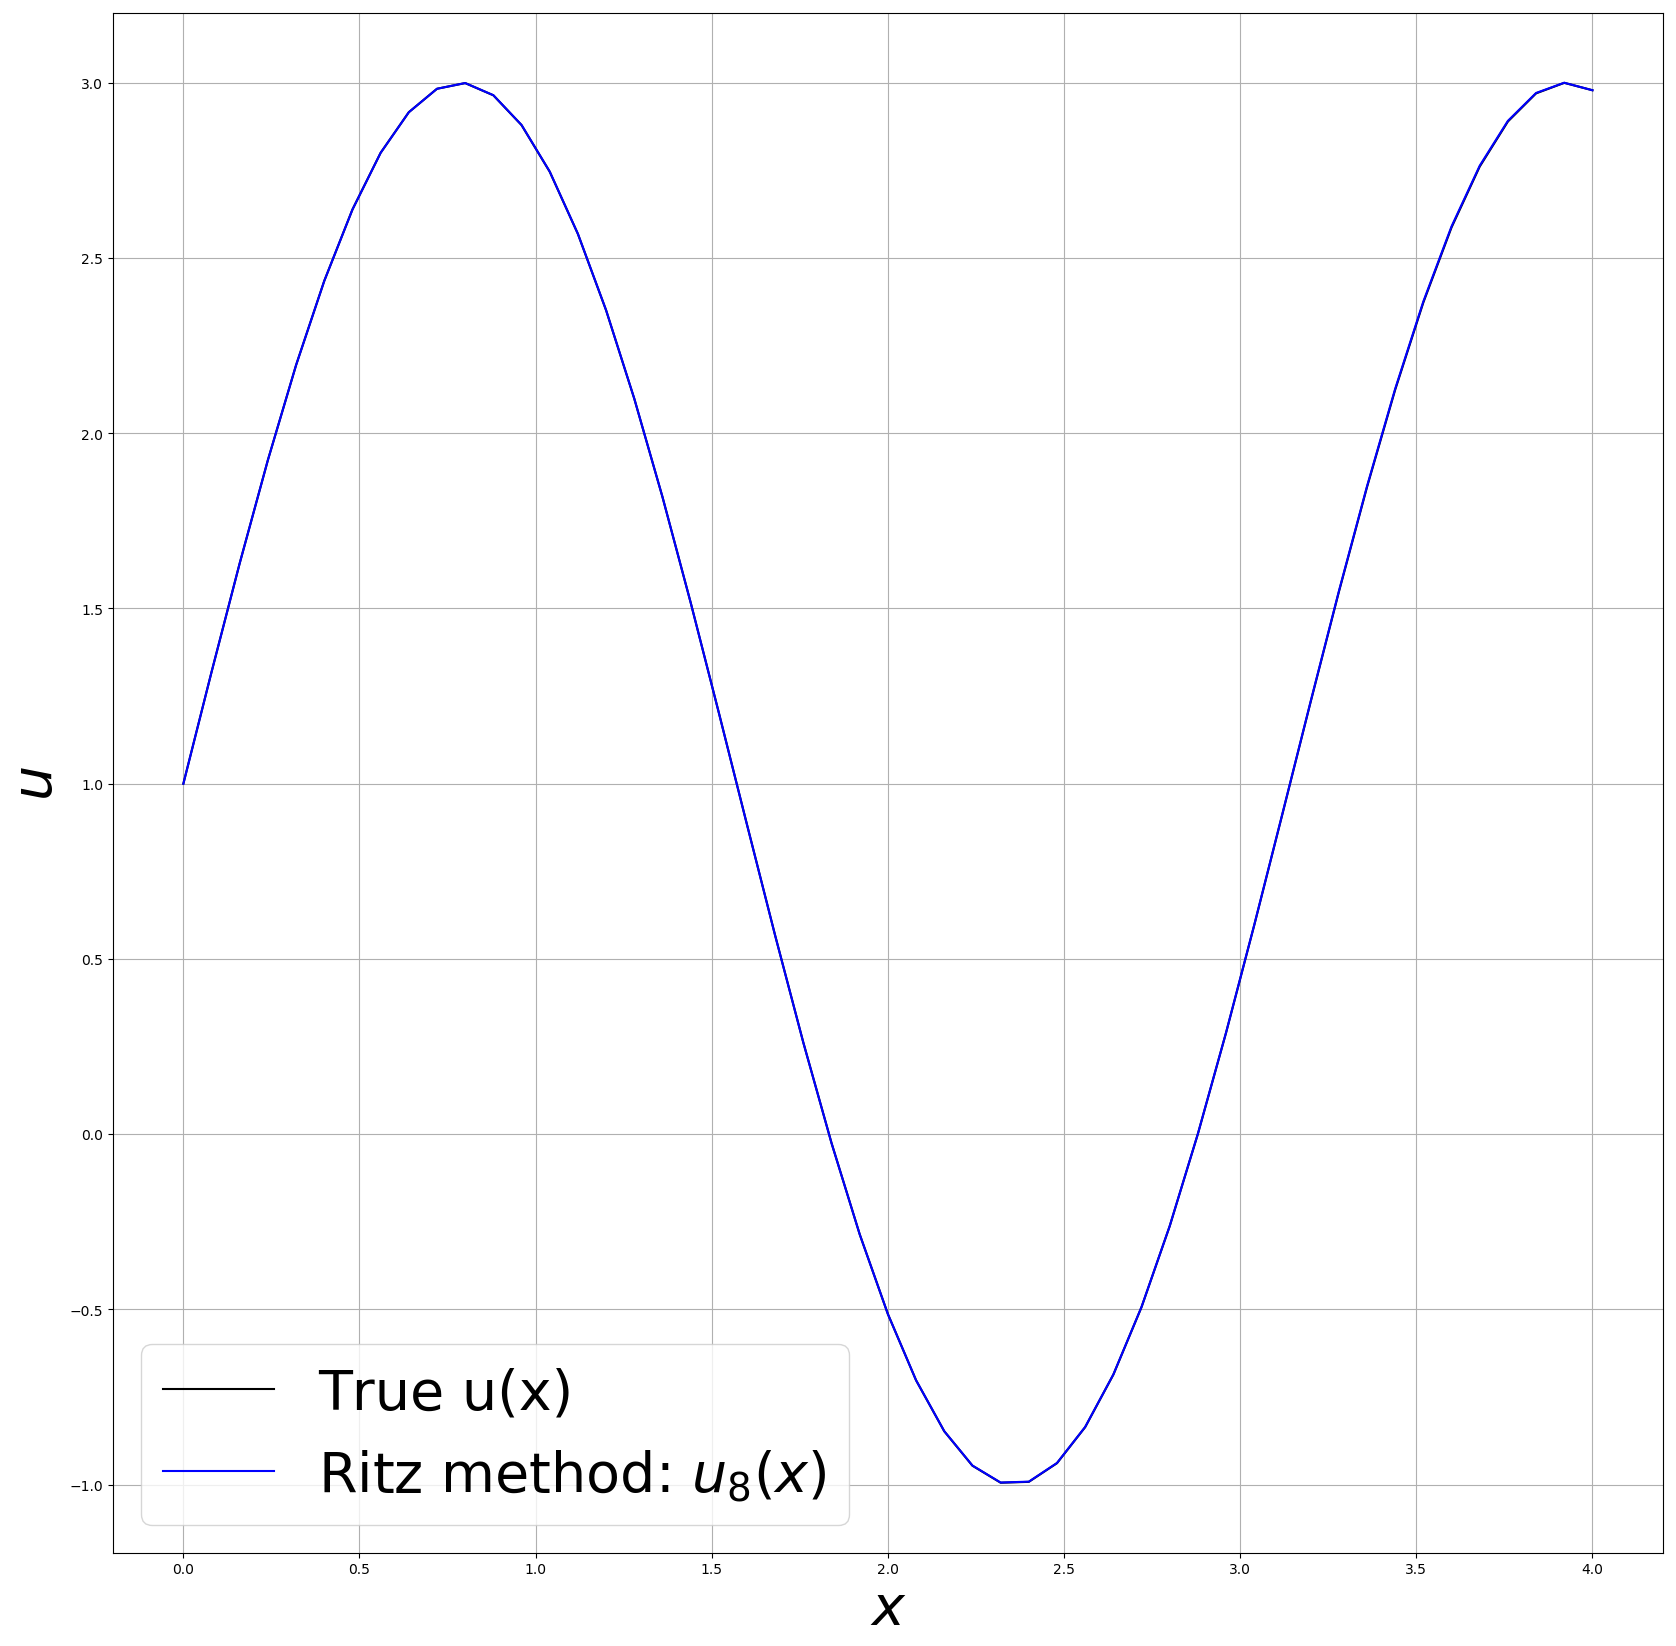
\includegraphics[width=.95\linewidth]{ritz_8.png}
    \caption{Рітца, 8 функцій}
    \end{subfigure}
\end{figure}

\end{document}
